%Need another paragraph to begin the description of these basics.
All regular instructions involving CPU computation within the
virtual machines are executed similarly to the physical machine
case, since no
switch between kernel and user modes is required during execution of
CPU instructions. However, in case of I/O operations, not only are
context switches between kernel and user modes required,
but also permissions and security are of paramount importance.
Basically, I/O operations have a higher access level
than CPU operations, and hence it is necessary for the Hypervisor
to intercept and arbitrate the I/O operations requested 
by the virtual machines. In this section, we present 
a brief background on I/O virtualization techniques, towards
setting up the background for work done in this thesis.

\subsection{Network I/O virtualization}
Hypervisor technology can be broadly classified into two types: 
(i) Type I hypervisor---those that run directly on the hardware (eg Xen) and, 
(ii) Type II hypervisor---those that run hosted on an existing operating system (eg KVM).


\begin{figure}[t]
\centering
% 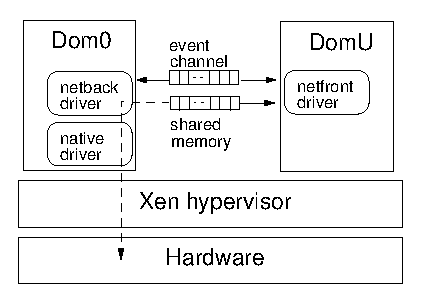
\includegraphics[height=1.75in]{jss-figures/xenarch.eps}
\hspace{-0.2in} \subfloat[Driver domain I/O model]{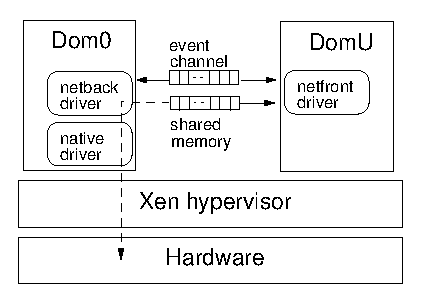
\includegraphics[scale=1]{jss-figures/xenarch.eps}} ~~~~~~~~~~~~~~~~~~~~
\subfloat[Direct I/O model]{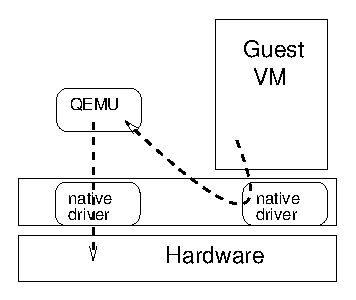
\includegraphics[scale=1]{jss-figures/kvmarch.eps}}
\caption{Different I/O virtualization architectures}%\textemdash{}}
\label{fig:xen-vs-kvm}
\end{figure}

%Xen~\cite{xen-art-of-virtualization} is a 
%para-virtualization\index{Para-virtualization} 
%based technology while KVM~\cite{kvm} is emulation based.
%\nomenclature{KVM:}{Kernel Virtual Machine}\index{KVM}
Xen~\cite{xen-art-of-virtualization} supports both full virtualization and 
para-virtualization---former using hardware-assisted virtualization technology
and latter using a privileged domain to arbitrate VM I/O operations.
Fig.~\ref{fig:xen-vs-kvm}(a) shows the Xen\index{Xen} 
para-virtualization architecture depicting 
Dom0\nomenclature{Dom0:}{Domain zero in Xen (driver domain)}\index{Dom0}\textemdash{}which 
is the privileged management/driver domain, and 
DomUs\nomenclature{DomU:}{User Domain in Xen (guest domain)}\index{DomU}\textemdash{}which 
are the guest virtual machines. 
All network I/O operations
of the guest VMs are arbitrated by Dom0 via a shared memory interface
termed Tx and Rx I/O rings. 
An event channel notification mechanism is used to notify events
to the domains, for example, notification to DomU regarding a 
received packet or notification to Dom0 for a packet to be
transmitted from DomU.
The \texttt{netfront}\index{Netfront} 
and \texttt{netback}\index{Netback} 
drivers, in DomU and Dom0 respectively,
coordinate the data exchange between the domains,
and the native driver in Dom0 coordinates exchange with
the physical network interface. 

%The above procedure is followed
%for both network operations as well as network-assisted disk I/O operations.
The I/O architecture used by Xen\index{Xen} with para-virtualization 
is known as the Driver domain I/O model. 
When the NIC receives a packet, it throws an interrupt that is caught by
the Xen hypervisor. The hypervisor removes the packet and forwards it
to the software bridge, which in turn, de-multiplexes the packet 
and delivers it to the backend of the appropriate VM. The backend
raises a hypercall for page remapping, after which the packet is 
delivered to the target VM. Similar process in reverse is applied
for a packet to be transmitted.

KVM~\cite{kvm} also supports both full virtualization and
para-virtualization---former wherein I/O
processing is done by the QEMU~\cite{qemu}\index{QEMU} emulator in 
userspace\index{KVM}\cite{kvm-whitepaper}
and latter using virtio framework~\cite{virtio}.
In emulated I/O architecture, there is no separate driver domain to handle 
privileged instructions, hence it is called 
the Direct I/O model~\cite{net-fairness-visa-2010}.
% performs dynamic binary translation of all guest
%instructions and executes them directly on the physical host hardware.
%This is called the Direct I/O model~\cite{net-fairness-visa-2010} and has no 
%separate
%driver domain to handle privileged instructions.
KVM/QEMU operates network I/O using TAP devices---a Linux kernel feature
that allows to create virtual network interfaces. When a packet is received,
the host NIC driver forwards it to the virtual bridge which de-multiplexes
and forwards it to the TAP device corresponding to the destination VM. 
When the TAP device receives data, it wakes up the QEMU process which
copies the data first into the VNIC buffer from where it gets copied 
into virtual device of the VM. Then QEMU process notifies kernel module
about the data, which in turn, sends interrupts to guest OS about data arrival.

Due to arbitration of DomU's I/O access by either the hypervisor or a
privileged domain, network activity of guest VMs results in additional
CPU utilization. However, since dispersed VMs communicate
by accessing the physical network interface as opposed to colocated VMs
that communicate ``locally'', network communication between
colocated and dispersed VMs results in different CPU overheads.
In the first component of our thesis, we study the CPU overheads
with colocation and dispersion of virtual machines and
build resource estimation models based on these findings.
\\
\\
In the above description, both Xen and KVM technologies are shown to 
have different I/O architectures, and the first component of our 
thesis deals with both architectures to demonstrate the difference
in CPU overheads for communicating VMs.
However, the \texttt{virtio}\index{Virtio} framework 
is a generic, modular and pluggable 
platform that can be used transparently with 
any hypervisor. The motivation for this framework was to
make hypervisor development
independent from the development of virtualization-based 
I/O drivers~\cite{virtio}. Also, it provides better performance
because it reduces the number of data copies and context switches.
This new framework shaped the design of our disk I/O redirection system
in the second component of this thesis, as explained next.

\subsection{Disk I/O virtualization}
A virtual machine's storage is called a virtual disk, can be either
an image file or a block device~\cite{ip-networked-storage}, and can be 
located on either a local disk attached to the 
physical machine, or network-attached as well.
When the virtual disk is located on a locally attached disk on the 
physical machine, it is referred to as Direct-attached 
storage (DAS)\nomenclature{DAS:}{Direct-attached Storage}\index{DAS},
whereas Network-attached storage (NAS)\index{NAS} and Storage Area Networks (SAN)\index{SAN}
are examples of storage that are accessible over the network.
Moreover, the difference between the virtual disk being a file or a
block device is that in case of a file, the virtual machine's ``disk-access
requests'' are translated into file-access requests by the Hypervisor, 
and then once again converted into block layer requests at the host
physical machine. This double-indirection is avoided in the case
where the virtual disk is itself a block device, and accessible using
block layer semantics, for 
eg. iSCSI\nomenclature{iSCSI:}{Internet Small Computer Systems Interface}\index{iSCSI}
SAN device~\cite{iscsi} or 
LVM-configured\nomenclature{LVM:}{Logical Volume Manager}\index{LVM}
storage volumes~\cite{lvm} on the physical machine.


%This section covers
%background related to disk I/O virtualization, and implications
%on host cache management.


\begin{figure}[t]
   \centering
   \subfloat[KVM]{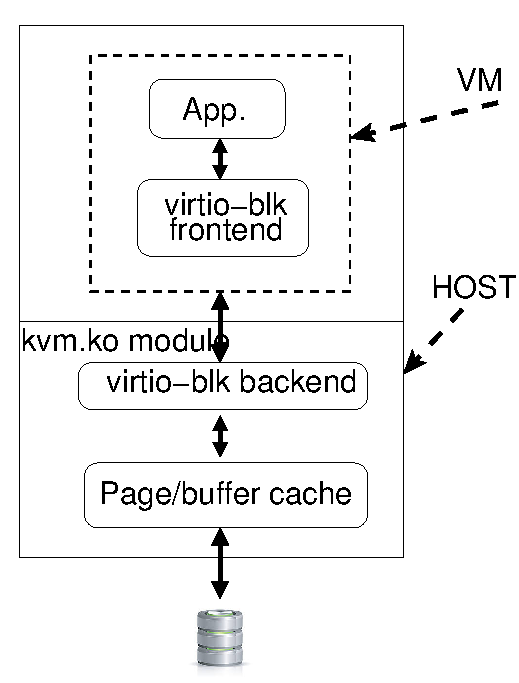
\includegraphics[scale=0.6]{confided-figures/main/kvm-disk-io.pdf}} ~~~~~~~~~~~~~~~
   \subfloat[Xen]{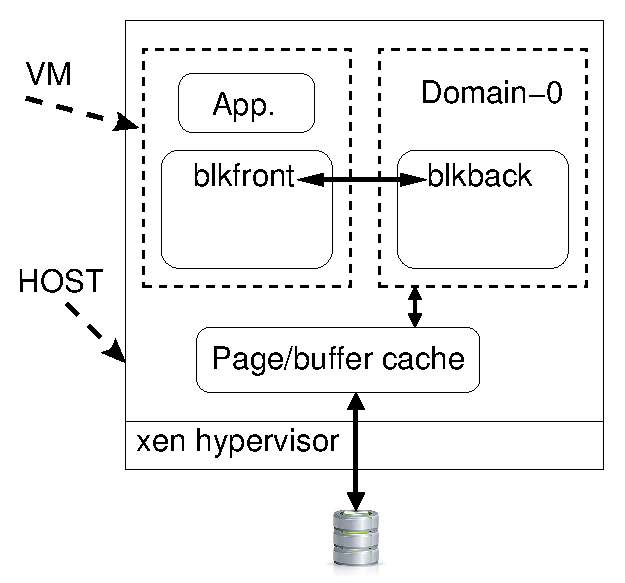
\includegraphics[scale=0.6]{confided-figures/main/xen-disk-io.pdf}} 
   \caption{Split-driver architecture for virtual block devices in KVM and Xen virtualization.}
   \label{fig:disk-io-arch}
%    \vspace{-0.2in}
\end{figure}

Irrespective of the type of storage used, the access to virtual disk is
performed via virtual block drivers within the VM. 
% In this sub-section, we 
% present background related to the paravirtualized virtual disk drivers,
% also referred as virtual block drivers.
As mentioned above, a new and emerging framework for 
virtual I/O device drivers is \texttt{virtio}~\cite{virtio}\index{virtio}. 
The basic concept of \texttt{virtio} is a split-driver
architecture, i.e., a pair of \texttt{frontend} 
and \texttt{backend} drivers that communicate with each other using
a ring-buffer mechanism.
The virtual machine hosts the \texttt{frontend} driver and forwards the
request to the corresponding \texttt{backend} driver hosted in the 
hypervisor or VMM\index{VMM}.
Virtio is developed in Hypervisor-agnostic fashion, with the only
constraint that Hypervisor and the guest OS are able to interact
with virtio using appropriate ring-buffer handling mechanisms.
Hence, virtio can be used
with a variety of Hypervisors like Xen, KVM and lguest virtualization 
solutions~\cite{virtio}.

The de-coupling of the virtual block device driver 
into \texttt{frontend}\index{Frontend} and \texttt{backend}\index{Backend} drivers
makes \texttt{virtio}
a generic virtual I/O mechanism, which can work on multiple hypervisors
and platforms. Currently, \texttt{virtio} is used as a high-performance
I/O mechanism in KVM~\cite{kvm}\index{KVM} virtualization technology. 
The paravirtualized block driver in Xen~\cite{xen} architecture also follows
the split-driver paradigm, wherein a privileged VM (Domain-0) hosts the 
\texttt{backend} driver. The split-driver architecture for virtual block devices
in Xen and KVM is illustrated in Fig.~\ref{fig:disk-io-arch}.
The communication between the \texttt{frontend} and \texttt{backend} block drivers is 
accomplished via a ring buffer transport mechanism, wherein each read
request is described in a descriptor placed into the ring buffers. Each
read request descriptor includes the block ID/address (to be read) and a 
buffer (into which the data is to be copied). 
In the second component of our thesis, we present a hint-based read
I/O redirection method positioned within the \texttt{frontend}
driver in a virtual machine, which can manipulate the downstream 
host cache in a content-deduplicated
fashion to improve its caching efficiency.
